% !TeX program = xelatex
% 第十七章 隐函数存在定理
\chapter{隐函数存在定理}

我们在第四章 §3 中曾给出了隐函数的概念及一元隐函数的微分法，在第十六章 §2 中又介绍了多元隐函数及隐函数组微分法．当时我们都是在隐函数（组）存在，且它们的导数或偏导数也存在的前提下进行的，即侧重点是求导方法，而存在性则默认．在这一章中，我们将把侧重点移到存在性问题，着重讨论在什么条件下隐函数（组）存在，并进一步讨论它们的连续性与可微性．

本章中定理的证明较长，但证明思路却是非常直观和清晰的．请读者注意借助几何图形来理解分析证明．

\section{单个方程的情形}

在第四章 §3 中，我们已经举例说明，对于二元函数 $z=F(x,y)$，方程
\begin{equation}
F(x,y)=0
\tag{1}
\end{equation}
有时确定唯一的一元隐函数 $y=f(x)$，有时确定多个一元隐函数，有时并不确定任何一元隐函数．本节将研究在什么条件下方程 $F(x,y)=0$ 确定唯一的隐函数．

注意方程（1）又可等价地表示为
\[
\left\{\begin{aligned}
z&=F(x,y),\\
z&=0,
\end{aligned}\right.
\]

\begin{figure}[htbp]
\centering
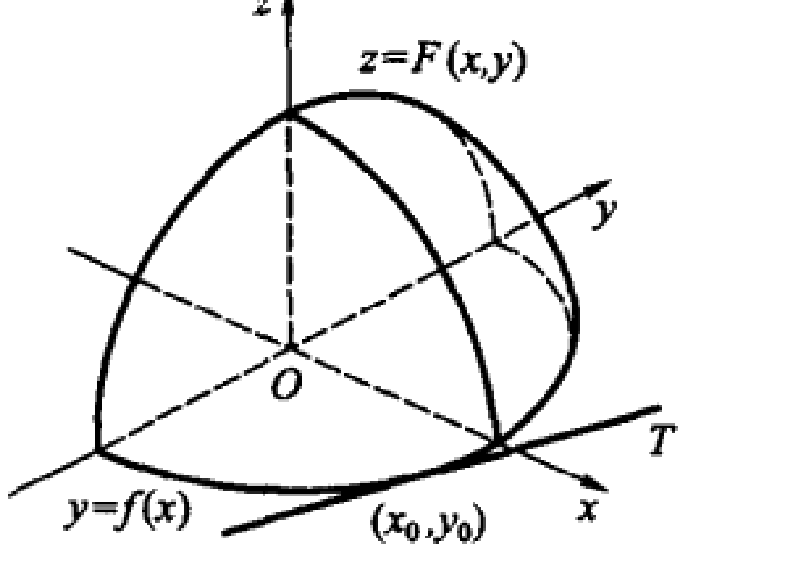
\includegraphics[width=0.45\textwidth]{work/figures/fig17-1}\caption{\relax}\label{fig:17-1}
\end{figure}

在几何上这是曲面 $z=F(x,y)$ 和坐标平面 $z=0$ 的交线．因此要使（1）式能确定隐函数，则曲面 $z=F(x,y)$ 必须与坐标面 $z=0$ 相交，也就是说，首先要存在 $P_{0}(x_{0},y_{0})$，使 $F(x_{0},y_{0})=0$．

进一步，如果希望这条过 $P_{0}$ 点的交线还是连续曲线的话，$F(x,y)$ 又应满足什么条件呢？如果曲面 $z=F(x,y)$ 在 $P_{0}$ 点有切平面，且切平面的法线不平行于 $z$ 轴，则切平面与坐标面 $z=0$ 相交为直线 $T$，这时 $z=F(x,y)$ 与 $z=0$ 必相交为曲线 $L$，且 $L$ 在 $P_{0}$ 点的切线就是 $T$．因为 $z=F(x,y)$ 在 $P_{0}$ 点的法向量为 $\left\{F_{x},F_{y},-1\right\}\big|_{P_{0}}$，所以切平面的法线不平行于 $z$ 轴意味着 $\left\{F_{x},F_{y},-1\right\}\big|_{P_{0}}$ 与 $\left\{0,0,1\right\}$ 不共线，即 $\left\{F_{x},F_{y}\right\}\big|_{P_{0}}\neq\left\{0,0\right\}$．另一方面，交线 $L$ 存在切线 $T$ 就意味着一元函数的可微性．因此条件 $\left\{F_{x},F_{y}\right\}\big|_{P_{0}}\neq\left\{0,0\right\}$ 不论对隐函数的存在性、连续性还是可微性都是重要的．下面的定理就从假定 $F_{y}\big|_{P_{0}}\neq0$ 入手．

\begin{theorem}\label{thm:17-1}
设 $F(x,y)$ 满足下列条件：

（i）$F_{x}$，$F_{y}$ 在 $D$: $\left|x-x_{0}\right|\leqslant a$，$\left|y-y_{0}\right|\leqslant b$ 上连续；

（ii）$F(x_{0},y_{0})=0$（通常称为初始条件）；

（iii）$F_{y}(x_{0},y_{0})\neq0$．

则

（1）存在 $\alpha>0$，使得在 $P_{0}$ 点的某一邻域内，方程 $F(x,y)=0$ 唯一地确定了一个定义在区间 $(x_{0}-\alpha,x_{0}+\alpha)$ 内的隐函数 $y=f(x)$，满足 $y_{0}=f(x_{0})$．换句话说，存在函数 $y=f(x)$，定义在 $(x_{0}-\alpha,x_{0}+\alpha)$ 内，满足 $F(x,f(x))\equiv0$，且 $y_{0}=f(x_{0})$；

（2）$y=f(x)$ 在 $(x_{0}-\alpha,x_{0}+\alpha)$ 连续；

（3）$y=f(x)$ 在 $(x_{0}-\alpha,x_{0}+\alpha)$ 有连续的导数，且
\[
f'(x)=-\frac{F_{x}(x,y)}{F_{y}(x,y)}.
\]
\end{theorem}

\begin{proof}
先注意一个事实，由条件（i），$F(x,y)$ 在 $D$ 上是连续的．下面分别证明各个结论成立．

由条件（iii），$F_{y}(x_{0},y_{0})\neq0$，不妨设 $F_{y}(x_{0},y_{0})>0$．又 $F_{y}(x,y)$ 在 $D$ 内连续，由连续函数的保号性，$F_{y}(x,y)$ 在 $(x_{0},y_{0})$ 点的某邻域内也大于零，为简便计，不妨设在 $D$ 上有 $F_{y}(x,y)>0$．因此对每一个 $x\in[x_{0}-a,x_{0}+a]$，$F(x,y)$ 关于 $y$ 在 $[y_{0}-b,y_{0}+b]$ 上是严格单调上升的．

固定 $x=x_{0}$，由条件（ii），$F(x_{0},y_{0})=0$ 以及 $F(x_{0},y)$ 在 $[y_{0}-b,y_{0}+b]$ 严格单调上升，知
\[
F(x_{0},y_{0}-b)<0,\ F(x_{0},y_{0}+b)>0.
\]
在 $F(x,y)$ 中分别固定 $y=y_{0}-b$ 和 $y=y_{0}+b$．由一元函数 $F(x,y_{0}-b)$，$F(x,y_{0}+b)$ 在 $x_{0}$ 连续，以及连续函数的保号性，知存在 $\alpha_{1}>0$（$\alpha_{1}<a$），使得当 $x\in(x_{0}-\alpha_{1},x_{0}+\alpha_{1})$ 时，有
\begin{equation}
F(x,y_{0}-b)<0;
\tag{2}
\end{equation}
存在 $\alpha_{2}>0$（$\alpha_{2}<a$），使得当 $x\in(x_{0}-\alpha_{2},x_{0}+\alpha_{2})$ 时，有

\begin{figure}[htbp]
\centering
\begin{tikzpicture}[scale=0.85]
% axes
\draw[-{Latex}] (-3.3,-2.1) -- (3.5,-2.1) node[below left] {$x$};
\draw[-{Latex}] (-3.3,-2.1) -- (-3.3,2.0) node[left] {$y$};
\node[below left] at (-3.3,-2.1) {$O$};
% rectangle D
\draw[thick] (-2.4,-1.5) rectangle (2.4,1.5);
% dashed guide lines: horizontal
\draw[dashed] (-3.3,1.5) -- (2.4,1.5);
\draw[dashed] (-3.3,0) -- (2.4,0);
\draw[dashed] (-3.3,-0.55) -- (2.4,-0.55);
\draw[dashed] (-3.3,-1.5) -- (2.4,-1.5);
% dashed guide lines: vertical
\draw[dashed] (-2.4,-2.1) -- (-2.4,1.5);
\draw[dashed] (-0.6,-2.1) -- (-0.6,1.5);
\draw[dashed] (0,-2.1) -- (0,1.5);
\draw[dashed] (2.4,-2.1) -- (2.4,1.5);
% inner rectangle sides x0-alpha, x0+alpha (solid, as in the book)
\draw[thick] (-1.5,-1.5) -- (-1.5,1.5);
\draw[thick] (1.7,-1.5) -- (1.7,1.5);
% curve y=f(x)
\draw[very thick] (-1.5,-0.95) .. controls (-1.05,-0.52) and (-0.9,-0.5) .. (-0.6,-0.55)
.. controls (-0.35,-0.62) and (-0.18,-0.25) .. (0,0)
.. controls (0.6,0.28) and (1.2,0.45) .. (1.7,0.55);
% labels on axes
\node[left] at (-3.3,1.5) {$y_0+b$};
\node[left] at (-3.3,0) {$y_0$};
\node[left] at (-3.3,-0.55) {$\overline{y}$};
\node[left] at (-3.3,-1.5) {$y_0-b$};
\node[below] at (-2.4,-2.15) {\scriptsize$x_0-a$};
\node[below] at (-1.5,-2.62) {\scriptsize$x_0-\alpha$};
\node[below] at (-0.6,-2.15) {\scriptsize$\overline{x}$};
\node[below] at (0,-2.62) {\scriptsize$x_0$};
\node[below] at (1.7,-2.15) {\scriptsize$x_0+\alpha$};
\node[below] at (2.4,-2.62) {\scriptsize$x_0+a$};
% point labels
\node[below right] at (-0.6,-0.55) {$\left(\overline{x},\overline{y}\right)$};
\node[above right] at (0,0) {$(x_0,y_0)$};
\node at (1.6,1.05) {$y=f(x)$};
\end{tikzpicture}\caption{\relax}\label{fig:17-2}
\end{figure}

\begin{equation}
F(x,y_{0}+b)>0.
\tag{3}
\end{equation}
令 $\alpha=\min(\alpha_{1},\alpha_{2})$，则当 $x\in(x_{0}-\alpha,x_{0}+\alpha)$ 时，（2），（3）式同时成立．

对任意 $\overline{x}\in(x_{0}-\alpha,x_{0}+\alpha)$，一元函数 $F(\overline{x},y)$ 在 $y\in[y_{0}-b,y_{0}+b]$ 连续，并且
\[
F(\overline{x},y_{0}-b)<0,\ F(\overline{x},y_{0}+b)>0.
\]
根据一元连续函数的介值定理，存在 $\overline{y}\in(y_{0}-b,y_{0}+b)$ 使得 $F(\overline{x},\overline{y})=0$，且由于 $F(\overline{x},y)$ 关于 $y$ 在 $[y_{0}-b,y_{0}+b]$ 严格单调上升，故使得 $F(\overline{x},\overline{y})=0$ 的 $\overline{y}\in(y_{0}-b,y_{0}+b)$ 是唯一的．这就确定了一个对应法则 $f$：对任意 $\overline{x}\in(x_{0}-\alpha,x_{0}+\alpha)$，都有唯一的 $\overline{y}\in(y_{0}-b,y_{0}+b)$ 与之对应，使得 $F(\overline{x},\overline{y})=0$．这就证明了，存在函数 $y=f(x)$，它定义在 $(x_{0}-\alpha,x_{0}+\alpha)$，满足 $F(x,f(x))=0$，特别地有 $y_{0}=f(x_{0})$．这样我们已经证明了结论（1）．

下面证结论（2）．既要证对任意 $\overline{x}\in(x_{0}-\alpha,x_{0}+\alpha)$，以及对任给的 $\varepsilon>0$，存在 $\delta>0$，$\delta$ 充分小使得 $(\overline{x}-\delta,\overline{x}+\delta)\subset(x_{0}-\alpha,x_{0}+\alpha)$，对任意 $x\in(\overline{x}-\delta,\overline{x}+\delta)$，有
\[
\left|f(x)-f(\overline{x})\right|<\varepsilon.
\]
任给 $\overline{x}\in(x_{0}-\alpha,x_{0}+\alpha)$，记 $\overline{y}=f(\overline{x})$．对任给的 $\varepsilon>0$，不妨设 $\varepsilon$ 充分小，使 $[\overline{y}-\varepsilon,\overline{y}+\varepsilon]\subset[y_{0}-b,y_{0}+b]$．因为 $y$ 的一元函数 $F(\overline{x},y)$ 在 $[\overline{y}-\varepsilon,\overline{y}+\varepsilon]$ 上严格单调上升，且 $F(\overline{x},\overline{y})=0$，所以
\[
F(\overline{x},\overline{y}-\varepsilon)<0,\ F(\overline{x},\overline{y}+\varepsilon)>0.
\]
而 $x$ 的一元函数 $F(x,\overline{y}-\varepsilon)$ 和 $F(x,\overline{y}+\varepsilon)$ 在 $x\in(x_{0}-\alpha,x_{0}+\alpha)$ 连续，故存在 $\delta_{1}>0$ 且 $(\overline{x}-\delta_{1},\overline{x}+\delta_{1})\subset(x_{0}-\alpha,x_{0}+\alpha)$，当 $x\in(\overline{x}-\delta_{1},\overline{x}+\delta_{1})$ 时有
\[
F(x,\overline{y}-\varepsilon)<0;
\]
存在 $\delta_{2}>0$ 且 $(\overline{x}-\delta_{2},\overline{x}+\delta_{2})\subset(x_{0}-\alpha,x_{0}+\alpha)$，当 $x\in(\overline{x}-\delta_{2},\overline{x}+\delta_{2})$ 时，有
\[
F(x,\overline{y}+\varepsilon)>0.
\]
令 $\delta=\min(\delta_{1},\delta_{2})$，则当 $x\in(\overline{x}-\delta,\overline{x}+\delta)$ 时，同时有
\[
F(x,\overline{y}-\varepsilon)<0,\ F(x,\overline{y}+\varepsilon)>0.
\]
因此只要 $x\in(\overline{x}-\delta,\overline{x}+\delta)$，$F(x,y)$ 作为 $y$ 的函数在 $(\overline{y}-\varepsilon,\overline{y}+\varepsilon)$ 就严格单调上升，且有唯一的零点 $y=f(x)$，显然满足
\[
y\in(\overline{y}-\varepsilon,\overline{y}+\varepsilon),
\]
即
\[
\left|f(x)-f(\overline{x})\right|<\varepsilon,
\]
结论（2）获证．

剩下来证明结论（3）．要证对任意 $\overline{x}\in(x_{0}-\alpha,x_{0}+\alpha)$，$y=f(x)$ 在 $\overline{x}$ 可导．令 $\left|\Delta x\right|$ 充分小使 $\overline{x}+\Delta x\in(x_{0}-\alpha,x_{0}+\alpha)$，记 $\overline{y}=f(\overline{x})$，$\overline{y}+\Delta y=f(\overline{x}+\Delta x)$．由 $y=f(x)$ 的定义知
\[
F(\overline{x},\overline{y})=0,\ F(\overline{x}+\Delta x,\overline{y}+\Delta y)=0.
\]
已知 $F(x,y)$ 在 $D$ 内有连续的偏导数，用二元函数的中值公式，存在 $\theta\in(0,1)$ 使得
\[
\begin{aligned}
0&=F(\overline{x}+\Delta x,\overline{y}+\Delta y)-F(\overline{x},\overline{y})\\
&=F_{x}(\overline{x}+\theta\Delta x,\overline{y}+\theta\Delta y)\Delta x+F_{y}(\overline{x}+\theta\Delta x,\overline{y}+\theta\Delta y)\Delta y.
\end{aligned}
\]
再由 $F_{x}$ 和 $F_{y}$ 的连续性及 $F_{y}(x,y)\neq0$，并注意到当 $\Delta x\to0$ 时 $\Delta y\to0$，便得
\[
\begin{aligned}
f'(\overline{x})&=\lim_{\Delta x\to0}\frac{\Delta y}{\Delta x}=\lim_{\Delta x\to0}-\frac{F_{x}(\overline{x}+\theta\Delta x,\overline{y}+\theta\Delta y)}{F_{y}(\overline{x}+\theta\Delta x,\overline{y}+\theta\Delta y)}\\
&=-\frac{F_{x}(\overline{x},\overline{y})}{F_{y}(\overline{x},\overline{y})}.
\end{aligned}
\]
这就是结论（3）．定理~\ref{thm:17-1} 证完．
\end{proof}

回顾定理的证明，不难看出，结论（2）的证明思路与结论（1）的证明思路完全相仿，几乎是将 $\overline{x}$，$\overline{y}$ 代替了 $x_{0}$，$y_{0}$ 后再重新叙述了一遍证明过程．其次，对于结论（1）、（2），定理条件（iii）可减弱为``$F(x,y)$ 在 $D$ 内关于 $y$ 是严格单调的''．但对结论（3），条件（iii）不能减弱．

在给出定理~\ref{thm:17-1} 之前，我们曾指出，条件 $\left\{F_{x},F_{y}\right\}\big|_{P_{0}}\neq\left\{0,0\right\}$ 不论对隐函数的存在性、连续性还是可微性都是重要的．这个条件等价于说 $F_{x}(x_{0},y_{0})\neq0$ 或 $F_{y}(x_{0},y_{0})\neq0$．考察定理~\ref{thm:17-1} 的条件，条件（i），（ii）关于 $x$，$y$ 是对称的，如果将条件（iii）改为 $F_{x}(x_{0},y_{0})\neq0$，则相应的全部结论成立，只是这时由 $F(x,y)=0$ 确定的隐函数是 $x=g(y)$．

\begin{example}\label{ex:17-1-1}
方程 $\cos y+\sin x=\mathrm{e}^{xy}$ 能否在原点的某邻域内确定隐函数 $y=f(x)$ 或 $x=g(y)$？
\end{example}

\begin{proof}[解]
令 $F(x,y)=\cos y+\sin x-\mathrm{e}^{xy}$，则
\[
F_{x}=\cos x-y\mathrm{e}^{xy},
\]
\[
F_{y}=-\sin y-x\mathrm{e}^{xy},
\]
它们都在全平面上连续，而
\[
F(0,0)=0,\ F_{x}(0,0)=1,\ F_{y}(0,0)=0,
\]
故方程在 $(0,0)$ 点的邻域内可唯一地确定可微的隐函数 $x=g(y)$，它定义在 $(-\alpha,\alpha)$，使得 $g(0)=0$，$F(g(y),y)=0$（$-\alpha<y<\alpha$）．但由于 $F_{y}(0,0)=0$，据此无法断定是否在 $(0,0)$ 点的某邻域内有隐函数 $y=f(x)$ 存在．

注意我们在这里用了``据此无法''这样的字眼，因为定理~\ref{thm:17-1} 的条件只是存在隐函数的充分条件，而不是必要条件．例如方程 $F(x,y)=y^{3}-x=0$，显然 $F_{y}(0,0)=0$，但仍可确定隐函数 $y=x^{\frac{1}{3}}$．
\end{proof}

\begin{example}\label{ex:17-1-2}
$F(x,y)=x^{2}+y^{2}-1$，$F_{x}=2x$，$F_{y}=2y$ 都在全平面连续．当 $y\neq0$ 时，$F_{y}\neq0$．由 $x^{2}+y^{2}-1=0$ 知，当 $y=0$ 时，$x=\pm1$．因此除 $(1,0)$ 和 $(-1,0)$ 点外，在单位圆上任何其它点 $(x_{0},y_{0})$，都存在 $(x_{0},y_{0})$ 的邻域，在这个邻域内可唯一确定可微的隐函数 $y=f(x)$．请读者思考，由方程可解出
\[
y=\sqrt{1-x^{2}}\quad\text{和}\quad y=-\sqrt{1-x^{2}},\ x\in(-1,1),
\]
这与隐函数存在的唯一性矛盾吗？
\end{example}

值得指出的是，定理~\ref{thm:17-1} 只肯定在 $x_{0}$ 的一个邻域，隐函数是存在的．我们说这是一个局部存在性的结果．隐函数在大范围的存在性，是个很复杂的问题，我们不在此讨论了．

现在再回头看看定理的证明，考察变量 $x$ 是否与它的维数有关．也就是说，如果将变量 $x$ 视为高维空间的点 $(x_{1},x_{2},\cdots,x_{n})$，定理的证明是否仍成立？我们发现的确成立，只要相应地把关于 $x$ 的区间改为邻域即可．

\begin{figure}[htbp]
\centering
\begin{tikzpicture}[scale=1.15]
\draw[-{Latex}] (-1.7,0) -- (1.9,0) node[below left] {$x$};
\draw[-{Latex}] (0,-1.7) -- (0,1.9) node[left] {$y$};
\node[below left] at (0,0) {$O$};
\draw[thick] (0,0) circle (1.25);
\draw (-0.35,1.08) rectangle (0.38,1.45);
\draw (-0.35,-1.45) rectangle (0.38,-1.08);
\draw (1.08,-0.35) rectangle (1.45,0.38);
\draw (-1.45,-0.35) rectangle (-1.08,0.38);
\node[right] at (0.15,1.18) {$(0,1)$};
\node[below] at (-1.25,-0.42) {$(-1,0)$};
\node[below] at (1.25,-0.42) {$(1,0)$};
\node[right] at (0.15,-1.4) {$(0,-1)$};
\end{tikzpicture}\caption{\relax}\label{fig:17-3}
\end{figure}

这样我们便可以将定理~\ref{thm:17-1} 推广到多元隐函数的情形．

\begin{theorem}\label{thm:17-2}
设函数 $F(x_{1},x_{2},\cdots,x_{n},y)$ 满足下列条件：

（i）偏导数 $F_{x_{i}}(i=1,2,\cdots,n)$ 和 $F_{y}$ 在 $D$: $\left|x_{i}-x_{i}^{(0)}\right|\leqslant a_{i}$（$i=1,2,\cdots,n$），$\left|y-y^{(0)}\right|\leqslant b$ 上连续，其中 $b>0$，$a_{i}>0$（$i=1,2,\cdots,n$）；

（ii）$F(x_{1}^{(0)},x_{2}^{(0)},\cdots,x_{n}^{(0)},y^{(0)})=0$；

（iii）$F_{y}(x_{1}^{(0)},x_{2}^{(0)},\cdots,x_{n}^{(0)},y^{(0)})\neq0$．

则

（1）存在 $Q_{0}(x_{1}^{(0)},x_{2}^{(0)},\cdots,x_{n}^{(0)})$ 的一个邻域 $O(Q_{0})$，使得在 $P_{0}(x_{1}^{(0)},x_{2}^{(0)},\cdots,x_{n}^{(0)},y^{(0)})$ 点的某邻域内，方程 $F(x_{1},x_{2},\cdots,x_{n},y)=0$ 唯一地确定了一个定义在 $O(Q_{0})$ 的 $n$ 元隐函数 $y=f(x_{1},x_{2},\cdots,x_{n})$，满足 $y^{(0)}=f(x_{1}^{(0)},x_{2}^{(0)},\cdots,x_{n}^{(0)})$．换句话说，存在函数 $y=f(x_{1},x_{2},\cdots,x_{n})$，$(x_{1},x_{2},\cdots,x_{n})\in O(Q_{0})$，使得当 $(x_{1},x_{2},\cdots,x_{n})\in O(Q_{0})$ 时，
\[
F(x_{1},x_{2},\cdots,x_{n},f(x_{1},x_{2},\cdots,x_{n}))\equiv0,
\]
且
\[
y^{(0)}=f(x_{1}^{(0)},x_{2}^{(0)},\cdots,x_{n}^{(0)});
\]

（2）$y=f(x_{1},x_{2},\cdots,x_{n})$ 在 $O(Q_{0})$ 内连续；

（3）$y=f(x_{1},x_{2},\cdots,x_{n})$ 在 $O(Q_{0})$ 内有连续的偏导数，且
\[
f_{x_{i}}=-\frac{F_{x_{i}}(x_{1},x_{2},\cdots,x_{n},y)}{F_{y}(x_{1},x_{2},\cdots,x_{n},y)},\ i=1,2,\cdots,n.
\]
\end{theorem}

\begin{example}\label{ex:17-1-3}
设 $\sin z-xyz=0$．问方程是否在原点 $(0,0,0)$ 的某邻域唯一地确定可微函数 $z=f(x,y)$，其中 $(x,y)$ 属于 $(0,0)$ 的某个邻域，使得 $\sin f(x,y)\equiv xyf(x,y)$．如可能，求 $\dfrac{\partial z}{\partial x}$，$\dfrac{\partial z}{\partial y}$．
\end{example}

\begin{proof}[解]
令 $F(x,y,z)=\sin z-xyz$．显然 $F(x,y,z)$ 在全平面有连续的偏导数，且 $F_{z}(x,y,z)=\cos z-xy$．由 $F_{z}(0,0,0)=1$，$F(0,0,0)=0$ 知，存在 $\alpha>0$，使得在 $\left|x\right|<\alpha$，$\left|y\right|<\alpha$ 有唯一的可微函数 $z=f(x,y)$，满足
\[
\sin f(x,y)=xyf(x,y),
\]
且
\[
\frac{\partial z}{\partial x}=-\frac{F_{x}(x,y,z)}{F_{z}(x,y,z)}=\frac{yz}{\cos z-xy},
\]
\[
\frac{\partial z}{\partial y}=-\frac{F_{y}(x,y,z)}{F_{z}(x,y,z)}=\frac{xz}{\cos z-xy}.
\]
\end{proof}

\begin{xiti}
\item 设函数 $F(x,y)$ 满足
\begin{ziti}
\item 在区域 $D$: $x_{0}-a\leqslant x\leqslant x_{0}+a$，$y_{0}-b\leqslant y\leqslant y_{0}+b$ 上连续；
\item $F(x_{0},y_{0})=0$；
\item 当 $x$ 固定时，函数 $F(x,y)$ 是 $y$ 的严格单调函数；
\end{ziti}
则可得到什么结论？试证明之．
\item 方程 $x^{2}+y+\sin(xy)=0$ 在原点附近能否用形如 $y=f(x)$ 的方程表示？又能否用形如 $x=g(y)$ 的方程表示？
\item 方程 $F(x,y)=y^{2}-x^{2}(1-x^{2})=0$ 在哪些点的附近可唯一地确定单值、连续、且有连续导数的函数 $y=f(x)$．
\item 证明有唯一可导的函数 $y=y(x)$ 满足方程 $\sin y+\sinh y=x$，并求出导数 $y'(x)$，其中 $\sinh y=\dfrac{\mathrm{e}^{y}-\mathrm{e}^{-y}}{2}$．
\item 方程 $xy+z\ln y+\mathrm{e}^{xz}=1$ 在点 $P_{0}(0,1,1)$ 的某邻域内能否确定出某一个变量是另外两个变量的函数．
\item 设 $f$ 是一元函数，试问 $f$ 应满足什么条件，方程
\[
2f(xy)=f(x)+f(y)
\]
在点 $(1,1)$ 的邻域内能确定出唯一的 $y$ 为 $x$ 的函数．
\item 设有方程：$x=y+\varphi(y)$，其中 $\varphi(0)=0$，且当 $-a<y<a$ 时，$\left|\varphi'(y)\right|\leqslant k<1$．证明：存在 $\delta>0$，当 $-\delta<x<\delta$ 时，存在唯一的可微函数 $y=y(x)$ 满足方程 $x=y+\varphi(y)$ 且 $y(0)=0$．
\end{xiti}

\section{方程组的情形}

关于由方程组决定的隐函数组的概念，在第十六章 §2 中已给出．下面以四个变量、两个方程的情形为例给出隐函数组存在定理．

\begin{theorem}\label{thm:17-3}
设函数 $F(x,y,u,v)$ 和 $G(x,y,u,v)$ 满足：

（i）在点 $P_{0}(x_{0},y_{0},u_{0},v_{0})$ 的某个邻域 $U$ 内，$F$，$G$ 对各变元有一阶连续偏导数；

（ii）$F(P_{0})=0$，$G(P_{0})=0$（初始条件）；

（iii）$J\big|_{P_{0}}=\dfrac{\partial(F,G)}{\partial(u,v)}\bigg|_{P_{0}}\neq0$．

则

（1）在 $P_{0}$ 点的某邻域 $\Delta\subset U$ 内，方程组
\begin{equation}
\left\{\begin{aligned}
F(x,y,u,v)&=0,\\
G(x,y,u,v)&=0
\end{aligned}\right.
\tag{1}
\end{equation}
唯一地确定一组函数 $u=u(x,y)$，$v=v(x,y)$，它们定义在 $(x_{0},y_{0})$ 的某邻域 $D$ 内，当 $(x,y)\in D$ 时，$(x,y,u,v)\in\Delta$，满足
\[
u_{0}=u(x_{0},y_{0}),\ v_{0}=v(x_{0},y_{0}),
\]
且
\[
\left\{\begin{aligned}
F(x,y,u(x,y),v(x,y))&\equiv0,\\
G(x,y,u(x,y),v(x,y))&\equiv0,
\end{aligned}\right.(x,y)\in D;
\]

（2）$u(x,y)$ 及 $v(x,y)$ 在 $D$ 内连续；

（3）$u(x,y)$ 及 $v(x,y)$ 在 $D$ 内有关于 $x$，$y$ 的连续偏导数，且
\[
\frac{\partial u}{\partial x}=-\frac{1}{J}\frac{\partial(F,G)}{\partial(x,v)},\quad \frac{\partial u}{\partial y}=-\frac{1}{J}\frac{\partial(F,G)}{\partial(y,v)},
\]
\[
\frac{\partial v}{\partial x}=-\frac{1}{J}\frac{\partial(F,G)}{\partial(u,x)},\quad \frac{\partial v}{\partial y}=-\frac{1}{J}\frac{\partial(F,G)}{\partial(u,y)}.
\]
\end{theorem}

\begin{proof}
反复应用定理~\ref{thm:17-2} 来证明．由条件（iii）
\[
\frac{\partial(F,G)}{\partial(u,v)}\bigg|_{P_{0}}=\begin{vmatrix}\dfrac{\partial F}{\partial u}&\dfrac{\partial F}{\partial v}\\[8pt]\dfrac{\partial G}{\partial u}&\dfrac{\partial G}{\partial v}\end{vmatrix}_{P_{0}}\neq0,
\]
知 $\left.\dfrac{\partial F}{\partial u}\right|_{P_{0}}$ 和 $\left.\dfrac{\partial F}{\partial v}\right|_{P_{0}}$ 至少有一个不为零，不妨设 $\left.\dfrac{\partial F}{\partial v}\right|_{P_{0}}\neq0$．由定理~\ref{thm:17-2}，方程 $F(x,y,u,v)=0$ 在 $P_{0}(x_{0},y_{0},u_{0},v_{0})$ 的某邻域内唯一地确定函数 $v=\varphi(x,y,u)$，它在 $(x_{0},y_{0},u_{0})$ 的某邻域 $V$ 内有连续的偏导数，且满足
\begin{equation}
v_{0}=\varphi(x_{0},y_{0},u_{0}),\quad F(x,y,u,\varphi(x,y,u))\equiv0.
\tag{2}
\end{equation}
记
\[
\psi(x,y,u)=G(x,y,u,\varphi(x,y,u)),\quad(x,y,u)\in V,
\]
则 $\psi(x,y,u)$ 在 $V$ 内有连续的偏导数，且 $\psi(x_{0},y_{0},u_{0})=0$．在方程组
\[
\left\{\begin{aligned}
\psi(x,y,u)&=G(x,y,u,\varphi(x,y,u)),\\
F(x,y,u,\varphi(x,y,u))&=0
\end{aligned}\right.
\]
中，两边对 $u$ 求偏导数，得
\[
\left\{\begin{aligned}
\psi_{u}&=G_{u}+G_{v}\varphi_{u},\\
F_{u}+F_{v}\varphi_{u}&=0.
\end{aligned}\right.
\]
解得
\[
\psi_{u}(x,y,u)=G_{u}-G_{v}\frac{F_{u}}{F_{v}}=-\frac{1}{F_{v}}\frac{\partial(F,G)}{\partial(u,v)}.
\]
由条件（iii）知 $\psi_{u}(x_{0},y_{0},u_{0})\neq0$，即 $\psi(x,y,u)$ 满足定理~\ref{thm:17-2} 的诸条件，从而方程
\[
G(x,y,u,\varphi(x,y,u))=0
\]
在 $(x_{0},y_{0},u_{0})$ 的某邻域内可唯一地确定函数 $u=u(x,y)$，它在 $(x_{0},y_{0})$ 的某邻域 $D$ 内有连续的偏导数，而当 $(x,y)\in D$ 时 $(x,y,u)\in V$，且满足
\[
u_{0}=u(x_{0},y_{0}),
\]
\begin{equation}
G(x,y,u(x,y)),\varphi(x,y,u(x,y))\equiv0.
\tag{3}
\end{equation}
令
\[
v(x,y)=\varphi(x,y,u(x,y)),\quad(x,y)\in D,
\]
则由（2）式知 $v(x,y)$ 在 $D$ 内有连续的偏导数，且
\begin{equation}
v_{0}=v(x_{0},y_{0}),\ F(x,y,u(x,y),v(x,y))\equiv0.
\tag{4}
\end{equation}
又由（3）式知
\begin{equation}
u_{0}=u(x_{0},y_{0}),\quad G(x,y,u(x,y),v(x,y))\equiv0,
\tag{5}
\end{equation}
即函数组 $u=u(x,y)$，$v=v(x,y)$ 就是由方程组（1）确定的满足定理要求（1）、（2）的函数组．最后只要证结论（3）中的公式成立．在（4）、（5）两式中两边对 $x$ 求偏导数，得
\[
\left\{\begin{aligned}
F_{x}+F_{u}\dfrac{\partial u}{\partial x}+F_{v}\dfrac{\partial v}{\partial x}&=0,\\[6pt]
G_{x}+G_{u}\dfrac{\partial u}{\partial x}+G_{v}\dfrac{\partial v}{\partial x}&=0.
\end{aligned}\right.
\]
用克拉默法则解出 $\dfrac{\partial u}{\partial x}$，$\dfrac{\partial v}{\partial x}$，即得
\[
\frac{\partial u}{\partial x}=-\frac{1}{J}\frac{\partial(F,G)}{\partial(x,v)},\quad \frac{\partial v}{\partial x}=-\frac{1}{J}\frac{\partial(F,G)}{\partial(u,x)}.
\]
同理在（4）、（5）两式中两边对 $y$ 求偏导数，得
\[
\frac{\partial u}{\partial y}=-\frac{1}{J}\frac{\partial(F,G)}{\partial(y,v)},\quad \frac{\partial v}{\partial y}=-\frac{1}{J}\frac{\partial(F,G)}{\partial(u,y)}.
\]
定理~\ref{thm:17-3} 证完．
\end{proof}

从定理~\ref{thm:17-3} 的证明中可见，条件（iii）在定理中的地位和作用与定理~\ref{thm:17-1} 中的条件 $F_{y}(x_{0},y_{0})\neq0$ 的地位和作用相当，它对于隐函数组的存在性、连续性和可微性都是重要的．另外，结论（3）中公式的推导方法就是我们在第十六章 §2 中介绍的隐函数组求导法，因此公式不必死记硬背，重要的是掌握求导方法．

\begin{example}\label{ex:17-2-1}
设有方程组
\[
\left\{\begin{aligned}
F(x,y,u,v)&=u^{2}+v^{2}-x^{2}-y=0,\\
G(x,y,u,v)&=-u+v-xy+1=0.
\end{aligned}\right.
\]
讨论在 $P_{0}(2,1,1,2)$ 的某邻域能否确定隐函数组 $u=u(x,y)$，$v=v(x,y)$．又问在 $P_{0}$ 点的某邻域能否确定函数组 $x=x(u,y)$，$v=v(u,y)$．对确定的函数组求其偏导数．
\end{example}

\begin{proof}[解]
显然 $F$，$G$ 在全平面上有连续的偏导数．又
\[
\begin{pmatrix}F_{x}&F_{y}&F_{u}&F_{v}\\ G_{x}&G_{y}&G_{u}&G_{v}\end{pmatrix}=\begin{pmatrix}-2x&-1&2u&2v\\ -y&-x&-1&1\end{pmatrix},
\]
\[
F(2,1,1,2)=0,\ G(2,1,1,2)=0,
\]
\[
\frac{\partial(F,G)}{\partial(u,v)}\bigg|_{P_{0}}=\begin{vmatrix}2u&2v\\ -1&1\end{vmatrix}_{P_{0}}=6\neq0,
\]
\[
\frac{\partial(F,G)}{\partial(x,v)}\bigg|_{P_{0}}=\begin{vmatrix}-2x&2v\\ -y&1\end{vmatrix}_{P_{0}}=0,
\]
因此在 $P_{0}$ 点的某邻域方程组可以唯一地确定一组可微函数 $u=u(x,y)$，$v=v(x,y)$，但在 $P_{0}$ 点的附近难以断言是否可唯一确定函数组 $x=x(u,y)$，$v=v(u,y)$．为求函数 $u(x,y)$ 和 $v(x,y)$ 的偏导数，在方程组两边对 $x$ 求偏导数，得
\[
\left\{\begin{aligned}
2u\frac{\partial u}{\partial x}+2v\frac{\partial v}{\partial x}-2x&=0,\\
-\frac{\partial u}{\partial x}+\frac{\partial v}{\partial x}-y&=0,
\end{aligned}\right.
\]
解得
\[
\frac{\partial u}{\partial x}=\frac{x-yv}{u+v},\quad \frac{\partial v}{\partial x}=\frac{yu+x}{u+v}.
\]
在方程组两边对 $y$ 求偏导数得
\[
\left\{\begin{aligned}
2u\frac{\partial u}{\partial y}+2v\frac{\partial v}{\partial y}-1&=0,\\
-\frac{\partial u}{\partial y}+\frac{\partial v}{\partial y}-x&=0,
\end{aligned}\right.
\]
解得
\[
\frac{\partial u}{\partial y}=\frac{1-2xv}{2(u+v)},\quad \frac{\partial v}{\partial y}=\frac{2xu+1}{2(u+v)}.
\]
\end{proof}

作为定理~\ref{thm:17-3} 的应用，我们考虑反函数组．

设有定义在平面点集 $D$ 上的函数组
\begin{equation}
u=u(x,y),\ v=v(x,y),\ (x,y)\in D,
\tag{6}
\end{equation}
则对于任意点 $(x,y)\in D$，都有平面上唯一的点 $(u,v)$ 与之对应．记 $D$ 的所有对应点的集合为 $D'$，即
\[
D'=\left\{(u,v)\mid(u,v)=(u(x,y),v(x,y)),\ (x,y)\in D\right\}.
\]
若反过来，对于任意点 $(u,v)\in D'$，都有唯一的点 $(x,y)\in D$，使得（6）式成立，也就是说，这时可确定两个定义在 $D'$ 上的函数
\begin{equation}
x=x(u,v),\ y=y(u,v),
\tag{7}
\end{equation}
在 $D'$ 上满足恒等式
\[
u\equiv u(x(u,v),y(u,v)),\quad v\equiv v(x(u,v),y(u,v)).
\]
则称函数组（7）是函数组（6）的反函数组．

上述对应关系可以用映射的语言加以叙述．我们称由（6）式给出的从 $D$ 到 $D'$ 的对应为映射 $T$：$D\to D'$，它把任意的 $(x,y)\in D$ 映为 $T(x,y)=(u,v)\in D'$．$D'$ 是 $D$ 在映射 $T$ 下的像集，记为 $D'=T(D)$．而（7）式则给出了从 $D'$ 到 $D$ 的映射 $T'$，它是 $T$ 的逆映射，即如果对任意的 $(u,v)\in D'$，有唯一的 $(x,y)\in D$，使得 $T(x,y)=(u,v)$，则说 $T'(u,v)=(x,y)$．这样的 $T'$ 存在的条件是：若 $(x_{1},y_{1}),(x_{2},y_{2})\in D$，且 $(x_{1},y_{1})\neq(x_{2},y_{2})$，则
\[
T(x_{1},y_{1})=(u_{1},v_{1})\neq T(x_{2},y_{2})=(u_{2},v_{2}).
\]
也就是说，$D$ 和 $D'$ 是一一对应的．$T$ 把 $D$ 映成 $D'$，而依同一关系，$T'$ 把 $D'$ 映回 $D$．这时记 $T'$ 为 $T^{-1}$．显然
\[
T^{-1}(T(x,y))=T^{-1}(u,v)=(x,y),\ (x,y)\in D,
\]
\[
T(T^{-1}(u,v))=T(x,y)=(u,v),\ (u,v)\in D'.
\]
因此，若 $T^{-1}$ 是 $T$ 的逆映射，则 $T$ 是 $T^{-1}$ 的逆映射．即 $T$ 与 $T^{-1}$ 互为逆映射．也就是说（6）、（7）式给出的函数组互为反函数组．

令
\[
\left\{\begin{aligned}
F(x,y,u,v)&=u-u(x,y)=0,\\
G(x,y,u,v)&=v-v(x,y)=0,
\end{aligned}\right.
\]
对 $F$ 和 $G$ 用定理~\ref{thm:17-3}，便得下面的反函数组定理．

\begin{theorem}\label{thm:17-4}
设函数组（6）满足

（i）在 $P_{0}(x_{0},y_{0})$ 的某邻域 $D$ 内对 $x$，$y$ 有连续偏导数；

（ii）$u_{0}=u(x_{0},y_{0})$，$v_{0}=v(x_{0},y_{0})$；

（iii）$\dfrac{\partial(u,v)}{\partial(x,y)}\bigg|_{(x_{0},y_{0})}\neq0$．

则在 $Q_{0}(u_{0},v_{0})$ 的某邻域 $D'$ 内存在唯一的一组反函数 $x=x(u,v)$，$y=y(u,v)$ 使得

（1）$x_{0}=x(u_{0},v_{0})$，$y_{0}=y(u_{0},v_{0})$，且当 $(u,v)\in D'$ 时 $(x,y)\in D$，有
\[
u\equiv u(x(u,v),y(u,v)),
\]
\[
v\equiv v(x(u,v),y(u,v));
\]

（2）$x(u,v)$，$y(u,v)$ 在 $D'$ 内存在连续的一阶偏导数，且
\[
\frac{\partial x}{\partial u}=\frac{1}{J}\frac{\partial v}{\partial y},\quad \frac{\partial x}{\partial v}=-\frac{1}{J}\frac{\partial u}{\partial y},
\]
\[
\frac{\partial y}{\partial u}=-\frac{1}{J}\frac{\partial v}{\partial x},\quad \frac{\partial y}{\partial v}=\frac{1}{J}\frac{\partial u}{\partial x}.
\]
其中 $J=\dfrac{\partial(u,v)}{\partial(x,y)}$．
\end{theorem}

\begin{corollary}\label{cor:17-1}
在定理~\ref{thm:17-4} 的条件下有 $\dfrac{\partial(x,y)}{\partial(u,v)}\cdot\dfrac{\partial(u,v)}{\partial(x,y)}=1$．
\end{corollary}

\begin{proof}
由定理~\ref{thm:17-4} 的结论（2）有
\[
\begin{aligned}
\frac{\partial(x,y)}{\partial(u,v)}&=\begin{vmatrix}\dfrac{\partial x}{\partial u}&\dfrac{\partial x}{\partial v}\\[8pt]\dfrac{\partial y}{\partial u}&\dfrac{\partial y}{\partial v}\end{vmatrix}=\frac{1}{J^{2}}\begin{vmatrix}\dfrac{\partial v}{\partial y}&-\dfrac{\partial u}{\partial y}\\[8pt]-\dfrac{\partial v}{\partial x}&\dfrac{\partial u}{\partial x}\end{vmatrix}\\
&=\frac{1}{J^{2}}\begin{vmatrix}\dfrac{\partial u}{\partial x}&\dfrac{\partial u}{\partial y}\\[8pt]\dfrac{\partial v}{\partial x}&\dfrac{\partial v}{\partial y}\end{vmatrix}=\frac{1}{J},
\end{aligned}
\]
即
\[
\frac{\partial(x,y)}{\partial(u,v)}\cdot J=\frac{\partial(x,y)}{\partial(u,v)}\cdot\frac{\partial(u,v)}{\partial(x,y)}=1.
\]
推论~\ref{cor:17-1} 证完．
\end{proof}

推论~\ref{cor:17-1} 可视为一元反函数导数公式 $\dfrac{\dd y}{\dd x}\cdot\dfrac{\dd x}{\dd y}=1$ 的推广．

\begin{corollary}\label{cor:17-2}
设函数组 $u=u(x,y)$，$v=v(x,y)$ 在开集 $D$ 内有连续偏导数，且在 $D$ 内 $\dfrac{\partial(u,v)}{\partial(x,y)}$ 恒不为零，则由函数组定义的映射 $T:D\to T(D)$ 的像集 $T(D)$ 是 $uv$ 平面上的开集．
\end{corollary}

\begin{proof}
对任意 $Q_{0}(u_{0},v_{0})\in T(D)$，设 $Q_{0}$ 是 $P_{0}(x_{0},y_{0})$ 在映射 $T$ 下的像，即 $u_{0}=u(x_{0},y_{0})$，$v_{0}=v(x_{0},y_{0})$．由反函数组定理，在 $Q_{0}$ 点的某邻域 $O(Q_{0})$ 内，存在唯一的一组反函数 $x=x(u,v)$，$y=y(u,v)$，使得 $x_{0}=x(u_{0},v_{0})$，$y_{0}=y(u_{0},v_{0})$，当 $(u,v)\in O(Q_{0})$ 时，$(x,y)\in D$，且有恒等式
\[
u\equiv u(x(u,v),y(u,v)),\quad v=v(x(u,v),y(u,v)).
\]
即 $O(Q_{0})$ 内的每一点都是 $D$ 中某一点的像，故 $O(Q_{0})\subset T(D)$．这就证明了 $T(D)$ 是开集．推论~\ref{cor:17-2} 证完．
\end{proof}

\begin{corollary}\label{cor:17-3}
在推论~\ref{cor:17-2} 的条件下，设 $E\subset D$ 是任一有界闭集，则它的像集 $T(E)$（$\subset T(D)$）也是有界闭集，且 $E$ 的内点映射为 $T(E)$ 的内点，$E$ 的边界点映射为 $T(E)$ 的边界点．
\end{corollary}

\begin{proof}
由于 $u(x,y)$ 和 $v(x,y)$ 在有界闭集上连续，从而有界，即 $T(E)$ 是有界集．下证 $T(E)$ 是闭集．设 $(u_{0},v_{0})$ 是 $T(E)$ 的聚点，则存在 $T(E)$ 中异于 $(u_{0},v_{0})$ 的点列 $\{(u_{n},v_{n})\}$，使得 $\lim\limits_{n\to\infty}(u_{n},v_{n})=(u_{0},v_{0})$．即存在 $E$ 中的点列 $\{(x_{n},y_{n})\}$，使得
\[
u_{n}=u(x_{n},y_{n}),\ v_{n}=v(x_{n},y_{n}),\ n=1,2,\cdots,
\]
且
\[
\lim_{n\to\infty}(u_{n},v_{n})=\lim_{n\to\infty}\left(u(x_{n},y_{n}),v(x_{n},y_{n})\right)=(u_{0},v_{0}).
\]
由致密性定理知 $\{(x_{n},y_{n})\}$ 有收敛子列 $\{(x_{n_{k}},y_{n_{k}})\}$．记其极限为 $(x_{0},y_{0})$，则有
\[
\lim_{k\to\infty}(x_{n_{k}},y_{n_{k}})=(x_{0},y_{0}).
\]
由 $E$ 闭知 $(x_{0},y_{0})\in E$，而函数 $u(x,y)$ 和 $v(x,y)$ 在 $E$ 上连续，所以
\[
\begin{aligned}
(u_{0},v_{0})&=\lim_{k\to\infty}\left(u(x_{n_{k}},y_{n_{k}}),v(x_{n_{k}},y_{n_{k}})\right)\\
&=\left(u(x_{0},y_{0}),v(x_{0},y_{0})\right).
\end{aligned}
\]
这表明 $(u_{0},v_{0})\in T(E)$，即 $T(E)$ 是闭集．

对 $T$ 用推论~\ref{cor:17-2}，知 $T$ 将 $E$ 的内点映射为 $T(E)$ 的内点．若 $T$ 将 $E$ 的某个边界点 $(x',y')$ 映射为 $T(E)$ 的内点 $(u',v')$，由定理~\ref{thm:17-4} 及推论~\ref{cor:17-1} 知，在 $(u',v')$ 的某邻域内存在 $T^{-1}$ 满足推论~\ref{cor:17-2} 的条件，于是 $T^{-1}$ 将 $(u',v')$ 映射为 $E$ 的内点 $(x',y')$，这与 $(x',y')$ 是 $E$ 的边界点矛盾，故 $(u',v')$ 是 $T(E)$ 的边界点．推论~\ref{cor:17-3} 证完．
\end{proof}

\begin{example}\label{ex:17-2-2}
极坐标与直角坐标的变换为
\[
x=r\cos\theta,\quad y=r\sin\theta.
\]
因为
\[
\frac{\partial(x,y)}{\partial(r,\theta)}=\begin{vmatrix}\dfrac{\partial x}{\partial r}&\dfrac{\partial x}{\partial\theta}\\[8pt]\dfrac{\partial y}{\partial r}&\dfrac{\partial y}{\partial\theta}\end{vmatrix}=\begin{vmatrix}\cos\theta&-r\sin\theta\\ \sin\theta&r\cos\theta\end{vmatrix}=r,
\]
所以除 $r=0$ 即坐标原点 $(0,0)$ 外，变换的逆变换存在，即有
\[
r=r(x,y),\ \theta=\theta(x,y).
\]
且
\[
\frac{\partial(r,\theta)}{\partial(x,y)}=\frac{1}{\dfrac{\partial(x,y)}{\partial(r,\theta)}}=\frac{1}{r}.
\]
\end{example}

最后，我们将定理~\ref{thm:17-3} 推广到一般的情形，即 $n+m$ 个变量，$n$ 个方程的情形．

\begin{theorem}\label{thm:17-5}
设有 $n$ 个 $n+m$ 元函数 $F_{i}(x_{1},x_{2},\cdots,x_{m},y_{1},y_{2},\cdots,y_{n})$（$i=1,2,\cdots,n$），满足

（i）在点 $P_{0}(x_{1}^{(0)},\cdots,x_{m}^{(0)},y_{1}^{(0)},\cdots,y_{n}^{(0)})$ 的某邻域 $U$ 内有对各变元的连续偏导数；

（ii）$F_{i}(P_{0})=0$，$i=1,2,\cdots,n$；

（iii）$J=\dfrac{\partial(F_{1},F_{2},\cdots,F_{n})}{\partial(y_{1},y_{2},\cdots,y_{n})}\bigg|_{P_{0}}\neq0$．

则（1）在 $P_{0}$ 的某邻域内，方程组
\[
F_{i}(x_{1},\cdots,x_{m},y_{1},\cdots,y_{n})=0\quad(i=1,2,\cdots,n)
\]
唯一地确定函数组
\[
y_{i}=f_{i}(x_{1},x_{2},\cdots,x_{m})\quad(i=1,2,\cdots,n),
\]
它们定义在 $(x_{1}^{(0)},x_{2}^{(0)},\cdots,x_{m}^{(0)})$ 的某邻域 $D$ 内，使得
\[
y_{i}^{(0)}=f_{i}(x_{1}^{(0)},x_{2}^{(0)},\cdots,x_{m}^{(0)})\quad(i=1,2,\cdots,n),
\]
且当 $(x_{1},x_{2},\cdots,x_{m})\in D$ 时有恒等式
\[
F_{i}(x_{1},x_{2},\cdots,x_{m},f_{1}(x_{1},x_{2},\cdots,x_{m}),\cdots,f_{n}(x_{1},x_{2},\cdots,x_{m}))\equiv0;
\]

（2）这组函数 $f_{i}$（$i=1,2,\cdots,n$）在 $D$ 内连续；

（3）这组函数 $f_{i}$（$i=1,2,\cdots,n$）在 $D$ 内对各变元有连续的偏导数，且对 $x_{j}$（$j=1,2,\cdots,n$）的偏导数可由下面方程组解出．
\[
\frac{\partial F_{i}}{\partial x_{j}}+\frac{\partial F_{i}}{\partial y_{1}}\frac{\partial f_{1}}{\partial x_{j}}+\frac{\partial F_{i}}{\partial y_{2}}\frac{\partial f_{2}}{\partial x_{j}}+\cdots+\frac{\partial F_{i}}{\partial y_{n}}\frac{\partial f_{n}}{\partial x_{j}}=0,\ i=1,2,\cdots,n.
\]
\end{theorem}

\begin{example}\label{ex:17-2-3}
点 $(1,-1,2)$ 在方程 $x^{2}(y^{2}+z^{2})=5$ 及 $(x-z)^{2}+y^{2}=2$ 所表示的曲面上，证明在这点的一个邻域内，两曲面的交线能用形如 $z=f(x)$，$y=g(x)$ 的一对方程表示．并求 $\dfrac{\dd z}{\dd x}$ 和 $\dfrac{\dd y}{\dd x}$．
\end{example}

\begin{proof}[证明]
令
\[
\left\{\begin{aligned}
F(x,y,z)&=x^{2}(y^{2}+z^{2})-5,\\
G(x,y,z)&=(x-z)^{2}+y^{2}-2,
\end{aligned}\right.
\]
这时 $F(1,-1,2)=0$，$G(1,-1,2)=0$．显然 $F$，$G$ 在点 $P_{0}(1,-1,2)$ 的任何邻域内有连续的偏导数，且
\[
\begin{aligned}
\left.\frac{\partial(F,G)}{\partial(y,z)}\right|_{P_{0}}&=\begin{vmatrix}\dfrac{\partial F}{\partial y}&\dfrac{\partial F}{\partial z}\\[8pt]\dfrac{\partial G}{\partial y}&\dfrac{\partial G}{\partial z}\end{vmatrix}_{P_{0}}=\begin{vmatrix}2x^{2}y&2x^{2}z\\ 2y&-2(x-z)\end{vmatrix}_{P_{0}}\\
&=\begin{vmatrix}-2&4\\ -2&2\end{vmatrix}=4\neq0.
\end{aligned}
\]
由定理~\ref{thm:17-5}，在 $P_{0}$ 点的某邻域内可唯一确定隐函数组
\[
z=f(x),\quad y=g(x),
\]
它们定义在 $x_{0}=1$ 点的某邻域内，使得 $f(1)=2$，$g(1)=-1$ 且
\[
F(x,g(x),f(x))\equiv0,\quad G(x,g(x),f(x))\equiv0.
\]
这表明两曲面的交线在 $P_{0}$ 附近能用形如 $z=f(x)$，$y=g(x)$ 的一对方程表示．在方程组两边对 $x$ 求导得
\[
\left\{\begin{aligned}
2x(y^{2}+z^{2})+x^{2}(2yy'+2zz')&=0,\\
2(x-z)(1-z')+2yy'&=0,
\end{aligned}\right.
\]
即
\[
\left\{\begin{aligned}
x^{2}yy'+x^{2}zz'&=-x(y^{2}+z^{2}),\\
yy'-(x-z)z'&=-(x-z).
\end{aligned}\right.
\]
解这个关于 $y'$ 和 $z'$ 的线性方程组得
\[
y'=\frac{y^{2}z-xy^{2}+z^{3}-x^{2}z}{x^{2}y},
\]
\[
z'=\frac{x^{2}-xz-y^{2}-z^{2}}{x^{2}}.
\]
\end{proof}

\begin{xiti}
\item 试讨论方程组
\[
\left\{\begin{aligned}
x^{2}+y^{2}&=\dfrac{1}{2}z^{2},\\
x+y+z&=2
\end{aligned}\right.
\]
在点 $P_{0}(1,-1,2)$ 的附近能否确定形如 $x=f(z)$，$y=g(z)$ 的隐函数组．
\item 求下列函数组的反函数组的偏导数：
\begin{ziti}
\item 设 $u=x\cos\dfrac{y}{x}$，$v=x\sin\dfrac{y}{x}$，求 $\dfrac{\partial x}{\partial u}$，$\dfrac{\partial x}{\partial v}$，$\dfrac{\partial y}{\partial u}$，$\dfrac{\partial y}{\partial v}$；
\item 设 $u=\mathrm{e}^{x}+x\sin y$，$v=\mathrm{e}^{x}-x\cos y$，求 $\dfrac{\partial x}{\partial u}$，$\dfrac{\partial x}{\partial v}$，$\dfrac{\partial y}{\partial u}$，$\dfrac{\partial y}{\partial v}$．
\end{ziti}
\item 设 $u=\dfrac{x}{r^{2}}$，$v=\dfrac{y}{r^{2}}$，$w=\dfrac{z}{r^{2}}$，其中 $r=\sqrt{x^{2}+y^{2}+z^{2}}$．
\begin{ziti}
\item 试求以 $u,v,w$ 为自变量的反函数组；
\item 计算 $\dfrac{\partial(u,v,w)}{\partial(x,y,z)}$．
\end{ziti}
\item 设 $f_{i}$，$\varphi_{i}$ 连续可微，且
\[
F_{i}(x_{1},\cdots,x_{n})=f_{i}(\varphi_{1}(x_{1}),\varphi_{2}(x_{2}),\cdots,\varphi_{n}(x_{n}))\quad(i=1,2,\cdots,n).
\]
求 $\dfrac{\partial(F_{1},F_{2},\cdots,F_{n})}{\partial(x_{1},x_{2},\cdots,x_{n})}$．
\item 据理说明：在点 $(0,1)$ 附近是否存在连续可微函数 $f(x,y)$ 和 $g(x,y)$ 满足 $f(0,1)=1$，$g(0,1)=-1$，且
\[
\begin{aligned}
&\left[f(x,y)\right]^{3}+xg(x,y)-y=0,\\
&\left[g(x,y)\right]^{3}+yf(x,y)-x=0.
\end{aligned}
\]
\item 设
\[
\left\{\begin{aligned}
u&=f(x,y,z,t),\\
g(y,z,t)&=0,\\
h(z,t)&=0.
\end{aligned}\right.
\]
在什么条件下 $u$ 是 $x$，$y$ 的函数？求 $\dfrac{\partial u}{\partial x}$，$\dfrac{\partial u}{\partial y}$．
\item 设函数 $u=u(x)$ 由方程组
\[
\left\{\begin{aligned}
u&=f(x,y,z),\\
g(x,y,z)&=0,\\
h(x,y,z)&=0
\end{aligned}\right.
\]
所确定，求 $\dfrac{\dd u}{\dd x}$，$\dfrac{\dd^{2}u}{\dd x^{2}}$．
\item 设 $z=z(x,y)$ 满足方程组
\[
\left\{\begin{aligned}
f(x,y,z,t)&=0,\\
g(x,y,z,t)&=0.
\end{aligned}\right.
\]
求 $\dd z$．
\item 设
\[
\left\{\begin{aligned}
u&=f(x-ut,y-ut,z-ut),\\
g(x,y,z)&=0.
\end{aligned}\right.
\]
求 $\dfrac{\partial u}{\partial x}$，$\dfrac{\partial u}{\partial y}$．这时 $t$ 是自变量还是因变量？
\item 设 $(x_{0},y_{0},z_{0},u_{0})$ 满足方程组
\[
\left\{\begin{aligned}
f(x)+f(y)+f(z)&=F(u),\\
g(x)+g(y)+g(z)&=G(u),\\
h(x)+h(y)+h(z)&=H(u),
\end{aligned}\right.
\]
这里所有的函数假定有连续的导数．
\begin{ziti}
\item 说出一个能在该点邻域内确定 $x$，$y$，$z$ 作为 $u$ 的函数的充分条件；
\item 在 $f(x)=x$，$g(x)=x^{2}$，$h(x)=x^{3}$ 的情形下，上述条件相当于什么？
\end{ziti}
\item 设 $x=u$，$y=\dfrac{u}{1+uv}$，$z=\dfrac{u}{1+uw}$，取 $u$，$v$ 为新的自变量，$w$ 为新的因变量，变换方程
\[
x^{2}\frac{\partial z}{\partial x}+y^{2}\frac{\partial z}{\partial y}=z^{2}.
\]
\end{xiti}
